\documentclass[a4paper,12pt]{article}
\usepackage{xltxtra}
\setromanfont{PT Sans}
\newfontfamily{\J}{American Typewriter}
\usepackage{labels}
\LabelGridtrue
\LabelCols=3
\LabelRows=2
\numberoflabels=6

\begin{document}
\addresslabel{
\vspace{3cm}

{\J \Huge \bfseries tryalgo \#1}\bigskip

Résolution de problèmes algorithmiques

\vspace{1.5cm}

Rejoignez le club ACM\\
\textbf{jeudi} 10 septembre \textbf{à 18~h}\\
en salle \textbf{C411} ! (Cournot)\bigskip

{\hfill \small acm@lists.crans.org}
}

\addresslabel{

\centering 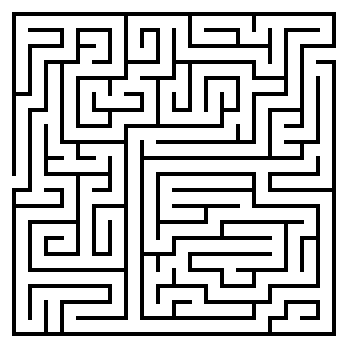
\includegraphics[width=0.5\linewidth]{maze.png}

\raggedright Comment déterminer un chemin vers la sortie ?\\[5mm]

\centering 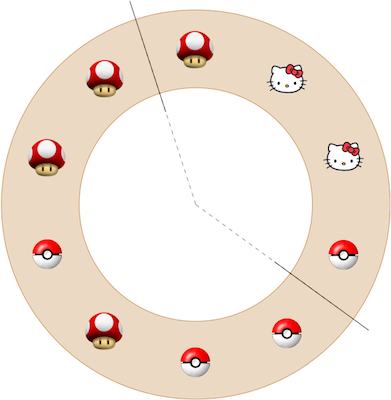
\includegraphics[width=0.55\linewidth]{epiphanie.png}

\raggedright Comment couper une plus petite part contenant tous les fruits confits ?\\[7mm]

\centering 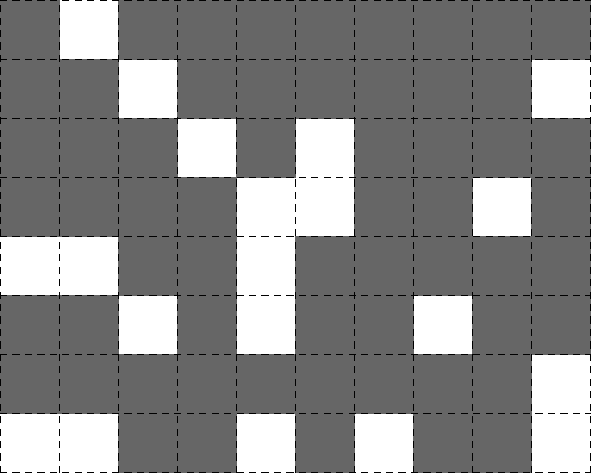
\includegraphics[width=0.5\linewidth]{rect}

\raggedright Comment trouver le plus grand carré tout noir ?}
\end{document}